%% approach

\section{Review of Previous Algorithms}
\label{sec:review}

Before presenting our algorithm, we start with reviewing existing approaches for maximal repeat enumeration. 



%%%%%% %% fig:CDAWG
\begin{figure}[t]
  \centering
  %% 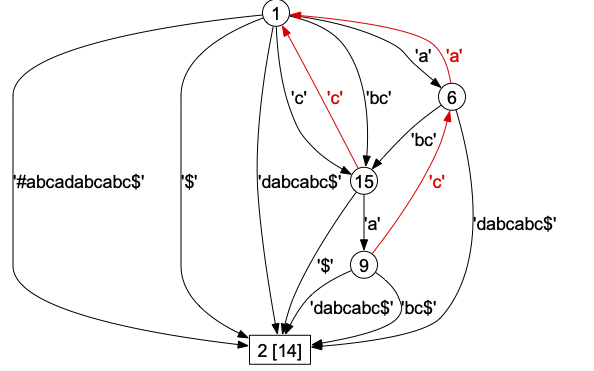
\includegraphics[height=0.4\textwidth]{fig/exp1/cdawg.pdf}
  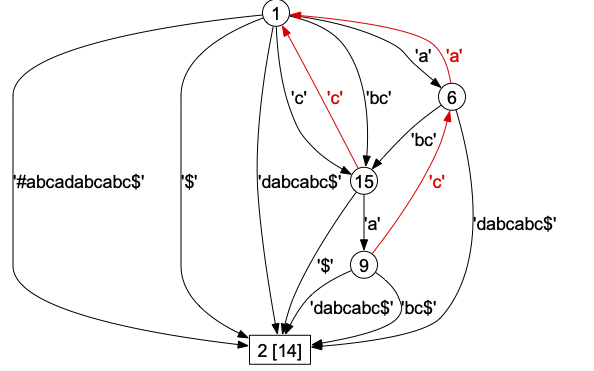
\includegraphics[height=0.4\textwidth]{fig/exp1/cdawg.png}
  \medskip 
  \caption{The CDAWG for a text $T = \mathtt{\#abcadabcabc\$}$ of length $13$. Its branching nodes $1, 6, 15$, and $9$ represents all of four maximal repeats $\eps, \mathtt{a}, \mathtt{abc}$, and $\mathtt{abca}$ with frequencies $14, 4, 3$, and $2$, respectively.
  }\label{fig:cdawg}
\end{figure}
%%%%%%


\subsection{Basics of enumerating maximal repeats}
Firstly, we explain the basic strategy of maximal repeat enumeration, which are common to all existing algorithms. 
Our result is obtained by combination of the top-down traversal of the virtual affix tree and efficient test for the left-branchingity based on the suffix array of a text. 
%%% 
We briefly explain our approach in the followings. 
%%We made a through survey of the existing algorithms for MR-enumeration. 

The CDAWG $\sig G$ for a txt $T$ (see \cref{fig:cdawg}) is a central data structure for dealing with  maximal repeats. It can be obtained from the suffix tree $\sig S$ (or equivalently its Weiner tree $\sig W$) for the same $T$ by merging all isomophic subtrees. Actually, what Raffinot~\cite{raffinot2001maximal} found was that that all nodes but the sink of the resuting DAG $G$, i.e., the CDAWG, represent all maximal repeats. 

On the other hand, if we view from the side of the suffix tree, all of its nodes with branching (outgoing) forward edges represent right-branching subwords of $T$, while all nodes with branching (incoming) backward edges (suffix links) represent left-branching subwords of $T$. Since maximal repeats are those subwords which are both left- and right-branching, we seek them by traversing either $\sig S$ or $\sig W$. 

Based on the above observation, we can classify enumeration algorithms by the following g two criteria: 
\begin{enumerate}[(1)]
\item The \textit{direction} of the traversal, i.e., either \textit{top-down} from the root to leaves~(\td), or \textit{bottom-up} from leaves to the root~(\bu). 
\item The \textit{types of edges} to follows, i.e., either \textit{forward}~(\fw) or \textit{backward}~(\bw). 
\end{enumerate}

\subsection{Classification of existing algorithms}

In \cref{table:summary}, we list and classify the state-of-the-art methods for MR enumeration ~\cite{narisawa2007efficient,okanohara2009linear,beller:berger2012space:efficient:bbo,belazzougui2020linear,nishimoto:cpm2021enum}. In the table, the last column ``Trav.~Type'' indicates the classification in combinations of tokens, such as $\tdfw$, the first one from $\set{\td, \bu}$ and the second one from $\set{\fw, \bw}$. 

By careful look at \cref{table:summary}, we found the existing algorithms fall into three groups below: 
\begin{enumerate}[(I)]
\item Three graph-based algorithms with type \tdfw, which has as an underlying structure either the suffix tree $\sig S$ or the CDAWG $\sig G$. 
There are no array-based algorithms with type \tdfw. 

\item Three array-based algorithms with type \tdbw, which has as an underlying structure is the Weiner tree $\sig W$. They traverse $\sig W$ based on the top-down simulation method proposed by Abouelhoda~\cite{abouelhoda2004replacing} using the BWT array and Wavelet tree. 


\item Two array-based algorithms with type \bufw, which has as an  underlying structure the suffix tree $\sig S$. They traverse $\sig S$ based on the bottom-up simulation method proposed by Kasai et al.~\cite{kasai:lee2001lcp:linear} 
using the SA and LCP arrays. 
\end{enumerate}

From the above classification, we can obtain some useful observation about the possible design of an efficient enumeration algorithm for MRs. 

\subsection{Analysis of the existing approaches}
%\subsection{Lessons learnt}
Firstly, all existing algorithms in group (I) are graph-based ones. Thus, they directly traverse the graph top-down by following forward edges without any difficulty. 
If the underlying graph $\sig G$ is isomorphic to the CDAWG of $T$, they can run in $O(e_R)$ time as desired. We can also see that there have been no existing array-based algorithms with type $\tdfw$ so far. We will come back to this issue later. 

Next, all existing array-based algorithms fall into the cases (II) and (III). 
For the case (II), algorithms has type \tdbw. They suffer from the fact that the underly tree $\sig W$ consists only of atomic backward edges. Therefore, the algorithms must traverse atomic backward edges one by one using the LF-mapping. From this reason, they must consume $\Theta(n)$ time by following a long chain of non-branching nodes until they  encounter a maximal repeat. 

For the case (III), algorithms has type \bufw. Unlike case (II), since all forward edges in the suffix tree $\sig S$ are path-compressed, they can avoid the problem with atomic edges. However, due to the bottom-up direction, they cannot make branch-and-bound search by pruning the useless subtrees. Consequently, they must travperse all of $\Theta(n)$ edges, resulting $\Theta(n)$ total running time. 

Finally, we are curious about this fact because we could not find any immediate reason by which we should avoid using the combination {\tdfw}, namely, the \textit{top-down search of the suffix tree $\sig S$ following forward edges}.  
Next, we will examine this approach further. 

\subsection{Our approach}
From the discussion in the previous subsection, the search strategy {\tdfw} seems a novel approach for efficient enumeration of maximal repeats. Actually, we can observe the following reasons to employ {\tdfw} as the basic strategy of our enumeration algorithm:  
\begin{enumerate}
\item \textit{Efficient pruning of non-maximal nodes}. Top-down search direction seems suitable to prune useless search paths than bottom-up search direction. This pruning should be efficiently done based on the left- or right-branchingity tests on indivisual nodes or subwords. This can be done by using the combination of the SA and LCP arrays with the help of the RMQ structure. 

\item \textit{Avoiding traversal of atomic edges}. Traversal with forward edges in $\sig S$ seems preferrable than that on backward edges in $\sig W$ to avoid traversal of atomic edges symbol by symbol. Since the path compression is closely related to the longest common prefixes of suffixes containing the locus of a subword, efficient test can be supported by  the LCP array with the RMQ structure, again. 
\end{enumerate}

We explain these ideas in the next section. 

%%% EOF
